\documentclass[conference]{IEEEtran}
\IEEEoverridecommandlockouts
% The preceding line is only needed to identify funding in the first footnote. If that is unneeded, please comment it out.
\usepackage{cite}
\usepackage{amsmath,amssymb,amsfonts}
\usepackage{algorithmic}
\usepackage{graphicx}
\usepackage{listings}
\usepackage{textcomp}
\usepackage{xcolor}
\usepackage{setspace}
\usepackage{array}
\usepackage{multirow}
\usepackage{tikz}
\usetikzlibrary{positioning,fit,shapes,arrows,calc}
\usetikzlibrary{arrows.meta}
\usepackage{hyperref}
\def\BibTeX{{\rm B\kern-.05em{\sc i\kern-.025em b}\kern-.08em
    T\kern-.1667em\lower.7ex\hbox{E}\kern-.125emX}}
    
\lstset{
  basicstyle=\ttfamily\small,
  columns=fullflexible,
  frame=single,
  breaklines=true,
  }
  
  
\tikzstyle{block} = [draw, rectangle, 
    minimum height=2em, minimum width=2em]
\tikzstyle{input} = [coordinate]
\tikzstyle{output} = [coordinate, node distance=1.2cm]
    
\begin{document}
\setstretch{1.0}

\title{State-of-the-art hyperparameter optimization methods}

\makeatletter
\newcommand{\linebreakand}{%
  \end{@IEEEauthorhalign}
  \hfill\mbox{}\par
  \mbox{}\hfill\begin{@IEEEauthorhalign}
}
\makeatother

\author{\IEEEauthorblockN{Marcell Molnár}
\IEEEauthorblockA{\textit{
Budapest University of Technology}\\
\textit{and Economics} \\
marcell.molnar97@gmail.com}
\and
\IEEEauthorblockN{Ákos Poleczki}
\IEEEauthorblockA{\textit{
Budapest University of Technology} \\
\textit{and Economics} \\
a.poleczki@gmail.com}
%\linebreakand 
%\IEEEauthorblockN{László Szerencsi}
%\IEEEauthorblockA{\textit{
%Budapest University of Technology}\\
%\textit{and Economics} \\
%laci.szerencsi@gmail.com}
}

\maketitle

\begin{abstract}
In this paper we discuss the currently available and most popular hyperparameter optimization (HPO) frameworks and methods. We start by defining the problem to be solved in the context of neural networks. Also, we present the state-of-the-art methods in details, how they work, and what thier advantages and disadvantages are. We showcase the Grid and Random Search algorithms, the Bayes Optimization technique, the Hyperband algorithm as well as the AutoML methods. Comparing these algorithms on multiple datasets is the final result of this work.
\end{abstract}

\begin{IEEEkeywords}
Deep Learning, Neural Networks, Hyperparameters, Hyperparameter Optimization
\end{IEEEkeywords}

\section{Introduction}
Optimizing hyperparameters is one of the most important tasks when striving for the best accuracy in any application. By changing some initialization parameters, for a given dataset, the resulting model is likely to achieve similar accuracy. However, modifying the structure of the model or the training parameters can lead to significantly different results.

In this paper, we are going to focus on optimizing the hyperparameters of neural networks, but the methods discussed  here can be easily extended to a variety of other Deep Learning topics as well. First, let’s clarify two terms:
\begin{itemize}
    \item \emph{Model parameters} are the variables in the models that are learned during the training process, e.g. the weights and biases in neural networks.
    \item \emph{Hyperparameters} are the parameters describing the structure of the network and the training method. For instance, the number of neurons in a layer, the number of hidden layers, or the type of activation function used.
\end{itemize}

\begin{figure}[htbp]
\centerline{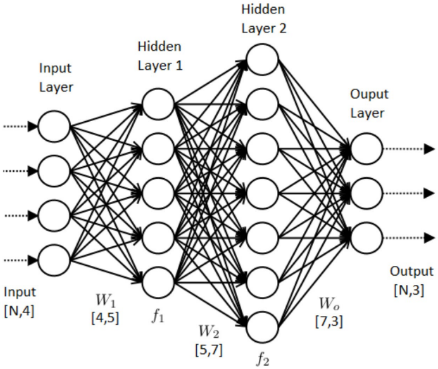
\includegraphics[width=0.4\textwidth]{nn.PNG}}
\caption{Typical neural network architecture. \cite{nn_arch} Model parameters are the weights ($W_{1}$, $W_{2}$ and $W_{o}$), hyperparameters are for example the number of hidden layers.}
\label{nn}
\end{figure}

Today, developers have the tools to automatically find the best values for the hyperparameters, meaning that the parameters themselves are derived through an extended learning process. Therefore, in these cases we can not distinguish between hyper- and model parameters, so different definitions are needed for the sake of our discussion.

The model parameters have a special property that is not present in the hyperparameters. We can calculate the derivatives of the neural network output error in regards to them. (For example, while iteratively updating them to get closer and closer to the optimal values, just like when the network is trained.) Meanwhile, we cannot do the same with the hyperparameters. Therefore, our new definition can be based on this property.

With that, we can further categorize the hyperparameters into two main groups. The ones which influence the architecture of the neural network, and the ones which used during the training phase. The most common hyperparameters in neural networks are:
\begin{enumerate}
    \item Model architecture parameters:
    \begin{itemize}
        \item Number of layers
        \item Number of neurons
    \end{itemize}
    \item Training parameters:
    \begin{itemize}
        \item Learning rate
        \item Batch size
        \item Activation function
        \item Optimization method (and its parameters)
        \item Droprate
    \end{itemize}
\end{enumerate}
(There are some other parameters, e.g. the Regularization method that can be modified and thus optimized to really fine tune the model.)

\section{Problem statement}
%https://towardsdatascience.com/hyperparameter-tuning-with-keras-and-ray-tune-1353e6586fda:
We can consider the hyperparameter tuning as a black-box optimization problem, where we are looking for the best x* input value that minimizes the function f(x), but without knowing the analytical form of f(x). These type of problems are also called derivative-free optimizations, because we are not able to calculate any derivatives due to the lack of knowledge of any analytical form of the objective function. Thus, methods like gradient descent and such neither can be applied here.
\begin{figure}[!ht]
		\centering
\begin{tikzpicture}[auto, node distance=0.1cm,>=latex',
  connection/.style={font=\fontsize{4}{4}}]
        \node[block] (blackbox) at (4.5,0) {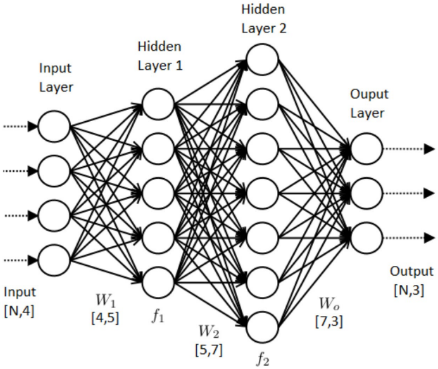
\includegraphics[width=.07\textwidth]{nn.png}};
        \node[block, align=center] (algo) at (0,0) {Hyperparameter\\Optimizer};
        \node [output, right=1.5cm of blackbox] (output) {};
        \draw [->] (algo.east) -- node [pos=0.5] {\small hyperparameters} (blackbox);
        \draw [->] (blackbox) -- node [name=feedback, pos=0.2] {} (output);
        \node (asdd) at ([yshift=0.2cm,xshift=1.0cm]blackbox.east) {accuracy,};
        \node (asde) at ([yshift=-0.2cm,xshift=1.0cm]blackbox.east) {loss, ...};
        \draw [draw,->] (feedback) --++ (0,-1.5cm) -| (algo.south);
\end{tikzpicture}
		\caption{Black-box optimization}
		\label{fig:simu_architecture}
\end{figure}

There are some known methods though, with which we can search for the best hyperparameter set, but the results are highly dependent on the input of the optimization problem. For every method, it is required to give the initial searching space, where we are trying to find the optimal solution. Thus, this interval should be large enough to surely contain the best value for each hyperparameter.
Unfortunately, the larger the search space, the greater the computational complexity too. So, in order to reduce the time needed for the optimization, it is recommended to select only the most influential parameters in the neural network.

Note that in the previous section, there were much less hyperparameters, which had an impact on the structure of the network, than which were affecting the training process. Due to this fact and with the aid of the preliminary knowledge of experts, the search space size for the network architecture can be reduced significantly. In the case of lacking expert experience, Automated Machine Learning (AutoML) has been proposed as a burgeoning technology to design and train neural networks automatically, at the cost of computational resources \cite{yu2020hyperparameter}.


\section{Algorithms for hyperparameter optimization}
\subsection*{Cross-validation}
Cross-validation is not really a hyperparameter optimization method, rather a technique to validate the model. A problem occurs when we train with a dataset and then we start changing the training based on a different, validation dataset. With that, we are making  changes so that the model produces good results on the latter dataset, instead of creating a well-generalized model. This often occures, when we deal with very diverse dataset, and use the same training and validation set for the whole training. Therefore, cross-validation uses one, large dataset to solve this problem. Partitioning the dataset at each epoch, will create different validation sets, which prevents the model from not being well-generalized.


\subsection{Grid Search}
Grid search is a basic method for hyperparameter optimization. It performs an exhaustive search on the hyperparameter set specified by the users. The users must have some preliminary knowledge on these hyper-parameters because it is they who generate all the candidates. Grid search is applicable for several hyper-parameters with limited search space.

Grid search is the most straightforward search algorithm that leads to the most accurate predictions. As long as sufficient resources are given, the user can always find the optimal combination \cite{grid_search_tds}. It is easy to run grid search in parallel because every trial runs individually without the influence of time sequence. Results for one trial are independent of those from other trials. Computational resources can be allocated in a highly flexible manner (see Figure \ref{grid}.). However, grid search suffers from the curse of dimensionality because the consumption of computational resources increases exponentially when more hyperparameters are awaiting tuning. Of course, methods exist for dimensionality reduction (e.g., PCA), but any method comes with a cost on the robustness of the model \cite{grid_search_tds_sec}. In addition, a limited sampling range is acceptable for grid search because too many configurations are not desirable. In practice, grid search is almost only preferable when users have enough experience of these hyperparameters to enable the definition of a narrow search space and no more than three hyperparameters need to be tuned simultaneously. \cite{yu2020hyperparameter}

\begin{figure}[htbp]
\centerline{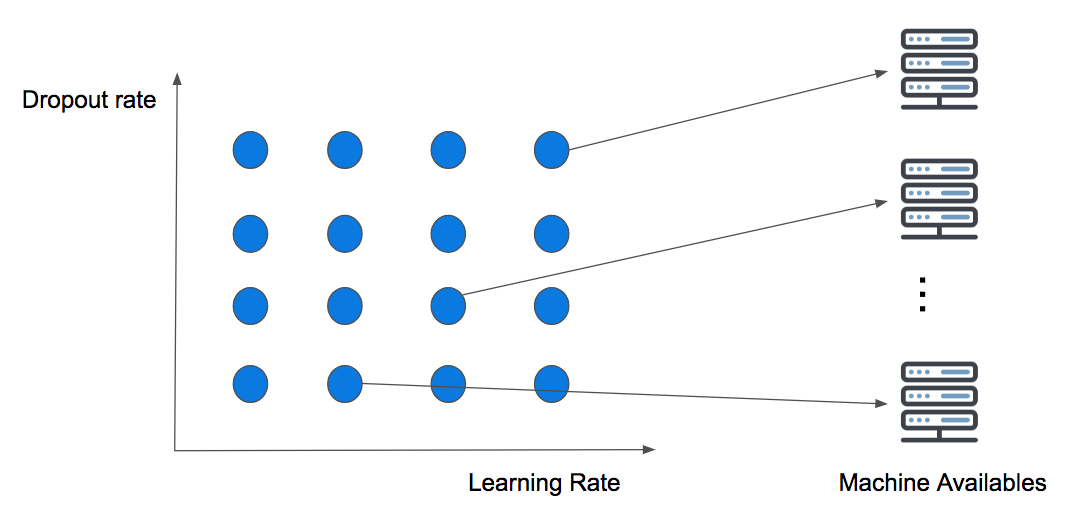
\includegraphics[width=0.5\textwidth]{grid.png}}
\caption{Grid Search parameter distribution over hyperparameters. \cite{grid_search} Configurations can be distributed over resources to reduce optimization time.}
\label{grid}
\end{figure}

Although other search algorithms may have more favorable features, grid search is still the most widely used method because of its mathematical simplicity. \cite{10.5555/2188385.2188395} \cite{yu2020hyperparameter}

\subsection{Random Search}
Random search \cite{10.5555/2188385.2188395} is a basic improvement on grid search. It indicates a randomized search over hyperparameters from certain distributions over possible parameter values. The searching process continues till the predetermined budget is exhausted, or until the desired accuracy is reached. Random search is similar to grid search but has been proven to create better results because of the following two benefits: first, a budget can be assigned independently according to the distribution of search space, whereas in grid search the budget for each hyperparameter set is a fixed value $B/N$ , where B is the total budget and N is the number of hyperparameters. Therefore, random search may perform better especially when some hyperparameters are not uniformly distributed. In this search pattern, random search is comparatively more likely to find the optimal configuration than grid search (see Figure \ref{grid_vs_random}.). Second, although obtaining the optimum using random search is not promising, it is quite certain that greater time consumption will lead to a larger probability of finding the best hyperparameter set. This logic is known as Monte Carlo technique, which is popular when dealing with large volume datasets in multi-dimensional deep learning scenarios \cite{10.1063/1.3295638}. By contrast, for grid search, a longer search time cannot guarantee better results. Easy parallelization and flexible resource allocation are also dominant advantages of random search \cite{10.5555/1981094.1981164}. \cite{yu2020hyperparameter}
\begin{figure}[htbp]
\centerline{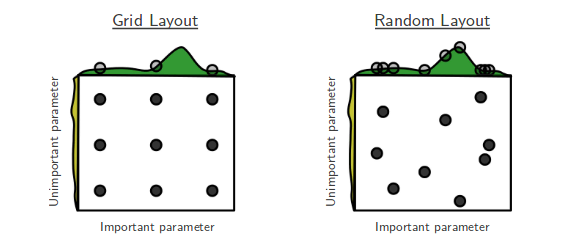
\includegraphics[width=0.5\textwidth]{grid_vs_random.png}}
\caption{Random Search search algorithm compared to Grid Search \cite{yu2020hyperparameter}. Random Search can deal with non uniformly distributed hyperparameters.}
\label{grid_vs_random}
\end{figure}

In most cases, random search is more effective than grid search, but it is still a computationally intensive method. The use of random search is suggested in the early stage of HPO to rapidly narrow down the search space, before using a guided algorithm to obtain a finer result (from a coarse to fine sampling scheme). Random search is often applied as the baseline of HPO to measure the efficiency of newly designed algorithms. Random search generally takes more time and computational resources than other guided search methods. \cite{yu2020hyperparameter}

\subsection{Bayes Optimization}
Bayesian optimization (BO) is a traditional algorithm with decades of history. It was raised by Jonas Mockus, and later became popular when it was applied to the global optimization problem \cite{jones}. BO is a typical method for almost all types of global optimization, and is aimed at becoming less wrong with more data. It is a sequential model-based method aimed at finding the global optimum with the minimum number of trials. It balances exploration and exploitation to avoid trapping into the local optimum. Exploitation is the process of making the best decision based on current information (Figure \ref{bayes}. right), whereas with exploration, the model will collect more information (Figure \ref{bayes}. left).
\begin{figure}[htbp]
\centerline{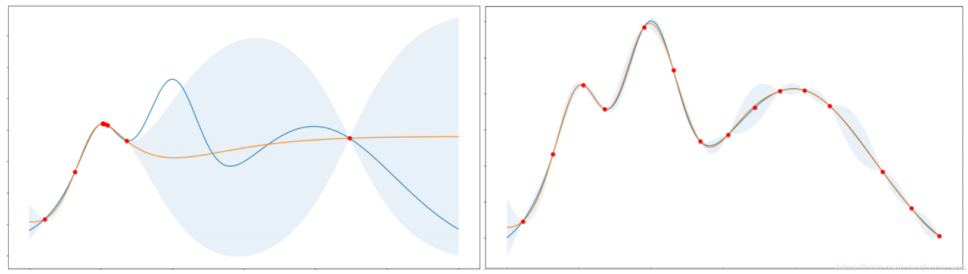
\includegraphics[width=0.5\textwidth]{bayes.png}}
\caption{Exploration-oriented (left) and exploitation-oriented Bayesian optimization (right). Shade indicates uncertainty. \cite{yu2020hyperparameter}}
\label{bayes}
\end{figure}

BO outperforms random search and grid search in two aspects: the first is that users are not required to possess preliminary knowledge of the distribution of hyperparameters, and the second is the posterior probability, which is the core idea of BO. The process of BO is described as follows: a probability surrogate model of objectives is built, and then every attempt is made based on the assessment of previous trials, and furthermore, the probability model is updated for the next trial until the most promising hyperparameter set is chosen. Compared with grid search and random search, BO is more computationally efficient with fewer attempts required to find the best hyperparameter set, in particular, especially when very costly objective functions are encountered. BO has another remarkable advantage over grid search and random search, it is applicable regardless of whether the objective function is stochastic or discrete, or convex or non-convex.

\subsection{HyperBand algorithm}
HyperBand is a novel algorithm for hyperparameter optimization published in 2018\cite{JMLR:v18:16-558} and has been added to Keras next year in 2019. The proposed approach focuses on speeding up random search through adaptive resource allocation and early-stopping. It formulates hyperparameter optimization as a pure-exploration non-stochastic infinite-armed bandit problem where a predefined resource like iterations, data samples, or features is allocated to randomly sampled configurations \cite{JMLR:v18:16-558}. Pure exploration bandit problems aim to minimize the simple regret, defined as the distance from the optimal solution, as quickly as possible in any given setting.

HyperBand algorithm involves the Successive Halving (SH) algorithm, which consists of four steps:
\begin{enumerate}
    \item Randomly sample $n$ pieces of hyperparameter configurations
    \item Evaluate the performances of all currently remaining configurations
    \item Throw out, the bottom half of the worst scoring configurations
    \item Go back to 2. and repeat until one configuration remains.
\end{enumerate}

HyperBand iteratively uses the Successive Halving algorithm with different input parameters, thus, SH is usually called the inner loop. In each (outer loop) run $n$ number of configurations are chosen, which are allocated with total of $R$ resources. The minimum resource that one configuration can receive is $r$. The outer loop starts from a high $n$, thus a small $r$. After every SH execution, $n$ is reduced, causing that each hyperparameter set can have more resources. This iteration is continued until the SH input is $n$=$1$ and $r$=$R$. The HyperBand algorithm returns the model with the best metrics seen in the whole search \cite{JMLR:v18:16-558}.



\subsection{AutoML}
Automated machine learning (AutoML) is a technique for automating the workflow from the raw data to the trained network. This workflow consists of the data preprocessing, feature engineering, model generation and model estimation.
\begin{figure}[htbp]
\centerline{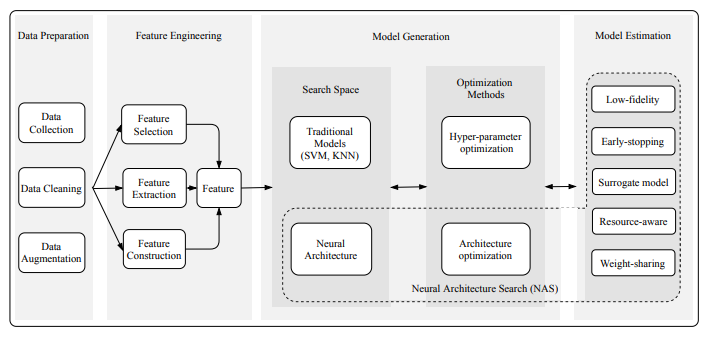
\includegraphics[width=0.5\textwidth]{automl.png}}
\caption{AutoML workflow \cite{he2020automl}}
\label{automl}
\end{figure}

Anyone, who has hands-on experience with neural networks, knows what the data preparation consists of. Once the raw data is collected, it should be cleaned, transformed to the same format, and augmented if needed. 

It is known that the dataset determines the upper bound of generalization capability of a neural network. Feature engineering aims to maximize the extraction of features from raw data for use by algorithms and
models. \cite{he2020automl}

Neural Architecture Search (NAS) is the process when we are trying to find the best structure of the network. The AutoML model has a defined Search Space where it is doing an Architecture Optimization. This is optimization is based on the Model Estimation when a generated network is evaluated.

The fourth component of AutoML is the hyperparamter optimization, when we are trying to maximize the accuracy for a given network. This is done through the algorithms discussed previously.

With AutoML, non-experts are also capable of creating neural networks with pretty good results.

\section{Popular hyperparameter optimization frameworks}
Altough many algorithms are available for hyperparameter optimization, the most used Deep Learning Frameworks only have implementation for a few methods, or just a wrapper for other libraries.

Tensorflow (not taking into account Keras in Tensorflow 2.0) only has a TensorBoard API that can show results of the hyperparameter optimization with the \emph{HParams Dashboard}. Thus, it has no algorithm for automated parameter tuning. The HParams Dashboard guide \cite{tensorboard} shows a grid search algorithm implemented by hand.

From Tensorflow version 2.0 we can use Keras as a built-in library. With that, we can use the \emph{Keras Tuner} framework to optimzie our model. Keras Tuner has implementation of Random Search, Bayesian Optimization and HyperBand algorithm.

We must note that there is an easy-to-use wrapper for hyperparameter optimization called Hyperas. It uses a the Tree-Structured Parzen Estimator (TPE) algorithm, which is a type of Bayes Optimization method.

The following popular framework is Scikit Learn, which uses Grid and Random Search, and with Scikit Optimize, we can use a wrapper to tune our model with Bayes Optimization.

RayTune is a Python library for experiment execution and hyperparameter tuning. It supports multiple machine learning frameworks, including PyTorch, XGBoost, MXNet, and Keras. The available algorithms are as Population Based Training (PBT), Bayes Optimization and HyperBand. PBT is similar to the evolutionary algorithms, when multiple instances of the network are present at the same time, and based on the entities \emph{fitness}, their parameters are propagated to the next generation of networks. \cite{jaderberg2017population}

There are also several AutoML frameworks available. Auto Sklearn, Google Cloud ML, AutoKeras, H2O AutoML, ML Box are just a few among many more. They provide easy to use APIs or graphical interfaces to create neural networks based on the input data.


\section{Related work}
\subsection{Data preparation}
Using Keras, we loaded the MNIST, Fashion MNIST, and CIFAR10 datasets that were used to test the HPO methods on. Then our data preparation consisted of three more steps. First, the data was  reshaped to the image sizes used in the dataset. Then, the normalization of the data followed, -  as the original data ranged from 0 to 255, which could lead to numerical problems, so  -  we divided each item by 255 so that we got a normalized dataset that do not cause problems. The final step was to divide the data into train, validation and test subgroups. We used 48000 train, 12000 validation and 10000 test images in the MNIST dataset, which gave about a 69\%-17\%-14\% ratio.
\begin{figure}[htbp]
\centerline{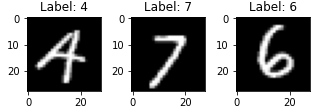
\includegraphics[width=0.35\textwidth]{mnist.png}}
\caption{Samples from the MNIST dataset}
\label{mnist}
\end{figure}\vspace{-1.0cm}
\begin{figure}[htbp]
\centerline{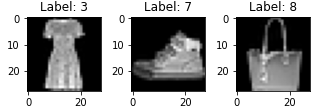
\includegraphics[width=0.35\textwidth]{fashion_mnist.png}}
\caption{Samples from the FASHION MNIST dataset}
\label{fashion_mnist}
\end{figure}\vspace{-0.5cm}
\begin{figure}[htbp]
\centerline{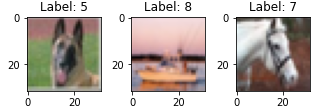
\includegraphics[width=0.35\textwidth]{cifar10.png}}
\caption{Samples from the CIFAR10 dataset}
\label{cifar10}
\end{figure}

\subsection{Data logging with TensorBoard}
When it comes to data visualization, TensorBoard is the way to go. It has a plenty of features to show datalogs, and also hyperparameter configurations.

The usage is simple and straightforward \cite{tensorboard}. First, we should configure tensorboard with and array of the hyperparameters and the metrics that will be logged.
\begin{lstlisting}[language=Python]
with tf.summary.create_file_writer(log_dir).as_default():
    hp.hparams_config(
        hparams=my_hparams,
        metrics=[hp.Metric('accuracy', display_name='Accuracy')]
    )
\end{lstlisting}
After the initialization, we can enter the training phase. After every training (and validation) we can write the current hyperparamters and the calculated metrics.
\begin{lstlisting}[language=Python]
with tf.summary.create_file_writer(log_dir).as_default():
    hp.hparams(current_hparams)
    tf.summary.scalar('accuracy', accuracy, step=1)
\end{lstlisting}

\subsection{Grid Search and Bayesian Optimization}
We used Scikit Learn's algorithms for the Grid Search and Bayesian Optimization. In order to be able to do the logging, we have created a custom \emph{KerasClassifier} class and used the inherited \emph{fit(..)} algorithm to get the current hyperparameters.
\begin{lstlisting}[language=Python]
class KerasRegressor_TensorBoardLogging(KerasClassifier):
    def __init__(self, *args, **kwargs):
        super(KerasRegressor_TensorBoardLogging, self).__init__(*args, **kwargs)

    def fit(self, x, y, **kwargs):
        hparams = self.get_params()
        with tf.summary.create_file_writer(get_logdir()).as_default():
            hp.hparams(hparams)
            super(KerasRegressor_TensorBoardLogging, self).fit(x, y, **kwargs)
\end{lstlisting}
\emph{KerasClassifier} is a wrapper class in Keras to use it in Scikit Learn's environment.

We also needed a custom callback to access the trained model's metrics. To do that, we inherited the Keras Callback class, and used it's \emph{on\_train\_end(..)} funciton.
\begin{lstlisting}[language=Python]
class MyHParamCallback(keras.callbacks.Callback):
    def on_train_end(self, logs=None):
        if log is not None:
            tf.summary.scalar('accuracy', logs['accuracy'], step=1)
\end{lstlisting}

\subsection{Random Search and HyperBand}
For Random Search and Hyperband algorithms, we used KerasTuner. Similar to Scikit Learn's case, we also needed here to inherit a class to be able to do the logging. The inherited classes are the \emph{RandomSearch} and the \emph{Hyperband}, which are Tuner classes in KerasTuner. At the end of every trail, we have access to the current hyperparameters, and the resulting metrics.
\begin{lstlisting}[language=Python]
class MyRandomSearchTuner(RandomSearch):
    def on_trial_end(self, trial):
        super().on_trial_end(trial)        
        with tf.summary.create_file_writer(log_dir).as_default():
            hparams = {
                key : trial.hyperparameters[key] for key in my_hparam_names
            }
            hp.hparams(hparams)
            tf.summary.scalar(METRIC_ACC, trial.score, step=1)
\end{lstlisting}

\subsection{Parameters and model to be optimized}
The hyperparameters we defined are the followings:
\begin{itemize}
    \item dropout : 0.0 to 0.4
    \item activation function : relu or sigmoid
    \item conv layer1 filters : 16, 32, 64 or 128
    \item conv layer2filters : 16, 32, 64 or 128
    \item dense layer neurons : 64, 128 or 256
    \item optimizer algorithm : SGD, RMSprop or Adam 
    \item learning rate : 0.001 or 0.01
\end{itemize}
Seeing these parameters, one can say that these are just a few variations in each hyperparameters, so we can easily find the best of them. The first half of this sentence is true, but sampling the dropout rate with 0.1, gives a total of 5$\times$2$\times$4$\times$4$\times$3$\times$3$\times$2=2880 combinations of hyperparameters. This already requires multiple days to test each of the combinations with just 10 epochs per model and with a mid - high-end GPU.

For every HPO methods, we need a function that returns with a compiled model using the given parameters.
\begin{lstlisting}[language=Python]
def create_tunable_model(dropout_rate = 0.0,
                         activation_fun = 'relu',
                         conv_layer1_filters = 32,
                         conv_layer2_filters = 32,
                         dense_layer_neurons = 128,
                         optimizer_algorithm = 'Adam',
                         learning_rate=0.001):
    model = Sequential()
    model.add(Conv2D(conv_layer1_filters, kernel_size=(3,3), activation=activation_fun, input_shape=(28,28,1) ))
    model.add(Conv2D(conv_layer2_filters, kernel_size=(3,3), activation=activation_fun ))
    model.add(MaxPool2D(pool_size=(2,2)))
    model.add(Dropout(dropout_rate))
    model.add(Flatten())
    model.add(Dense(dense_layer_neurons, activation=activation_fun))
    model.add(Dropout(dropout_rate))
    model.add(Dense(10, activation='softmax'))

    if optimizer_algorithm == 'Adam':
        optimizer_method = keras.optimizers.Adam(learning_rate=learning_rate)
    if optimizer_algorithm == 'RMSprop':
        optimizer_method = keras.optimizers.RMSprop(learning_rate=learning_rate)
    if optimizer_algorithm == 'SGD':
        optimizer_method = keras.optimizers.SGD(learning_rate=learning_rate)
       
    model.compile(loss='categorical_crossentropy', optimizer=optimizer_method, metrics=['accuracy'])
    return model
\end{lstlisting}

\section{Discussion and results}
Due to the fact that grid search is very ineffective algorithm, and its execution requires more days, we only checked it on the MNIST dataset. On the MNIST dataset, we also tested what happens if a systematic method (anything except Grid Search) runs for 120 or 1400 iterations. The results showed, that the best achieved accuracies and validation accuracies were almost the same, and the differences are negligible. With the Random Search algorithm, the best achieved accuracy was 99.79\% in 120 runs, and 99.82\% in 1400 runs. The 10th best models achieved 99.05\% and 99.18\% accuracies. The validation accuracies were close to the train accuracies. From this, we can conclude that 120 iterations are sufficient for the HPO. Thus, we have set Random Search algorithm's max iterations to 120, and then we tuned the other algorithms to run for about the same time as the Random Search did. We choose this solution, because HyperBand does not deal with full trains and consequently the same amount of training would result in worse accuracy.

\subsection{MNIST}
Now let's look at the results with the MNIST dataset.
\begin{table}[htbp]
	\footnotesize
	\renewcommand{\arraystretch}{1.0} % to increase cell height
\begin{center}
\begin{tabular}{|c|c|c|c|c|} \hline
	Method & Best acc & Best val acc & Best loss & Best val loss \\ \hline
	Grid Search & 99.915 & 98.892 & 0.0036708 & 0.091984 \\ \hline
	Random Search & 99.792 & 99.000 & 0.12749 & 0.069942 \\ \hline
	Bayes Opt & 99.821 & 98.600 & 0.0055018 & 0.077322 \\ \hline
	HyperBand & 98.822 & 98.904 & 0.17447 & 0.057610 \\ \hline
	\end{tabular}
	\label{tab:results_mnist}
\end{center}
	\caption{Comparison of the methods on the mnist dataset}
\end{table}

Because Grid Search tries every possible hyperparameter combinations, it will find the best parameter set, if the continuous parameters are sampled fine enough. This is true, because the best train accuracy was achieved by Grid Search, although other methods could reach better, quasi the same and almost the same validation accuracy. Thus, we can say that systematic methods are able to find a solution near to the global optima with way less execution time.

The Bayes optimization achieved the second best accuracy on the MNIST dataset, but the HyperBand and Random Search achieved a slightly better validation accuracy. From the values in Table I, we can say that the MNIST is a very-easy-to-learn dataset, models can reach very impressive results.

\subsection{Fashion MNIST}
\begin{table}[htbp]
	\footnotesize
	\renewcommand{\arraystretch}{1.0} % to increase cell height
\begin{center}
\begin{tabular}{|c|c|c|c|c|} \hline
	Method & Best acc & Best val acc & Best loss & Best val loss \\ \hline
	Random Search & 98.775 & 93.083 & 0.31435 & 0.38346 \\ \hline
	Bayes Opt & 99.267 & 92.742 & 0.021059 & 0.40492 \\ \hline
	HyperBand & 92.100 & 91.483 & 0.41605 & 0.34986 \\ \hline
	\end{tabular}
	\label{tab:results_fashionmnist}
\end{center}
	\caption{Comparison of the methods on the fashion mnist dataset}
\end{table}\vspace{-0.3cm}

Fashion MNIST is a similar dataset to MNIST, but can be harder the train a model on it. The Bayes optimization achieved again the best accuracy, but just slightly better than Random Search. The difference between the train and validation accuracies were much greater here, than on the MNIST dataset. The only exception for this, is the HyperBand's result, because it reached about the same train and validation accuracy.

\subsection{CIFAR10}
CIFAR10 is a more diverse dataset than the previous ones, furthermore it not a dataset with gray scaled images, instead an RGB ones. Also, the images in CIFAR10 are not cropped pictures, they have variable background and can have disturbing objects on them. Now, let's look at the best results.
\begin{table}[htbp]
	\footnotesize
	\renewcommand{\arraystretch}{1.0} % to increase cell height
\begin{center}
\begin{tabular}{|c|c|c|c|c|} \hline
	Method & Best acc & Best val acc & Best loss & Best val loss \\ \hline
	Random Search & 88.650 & 69.630 & 1.3964 & 1.1351 \\ \hline
	Bayes Opt & 94.549 & 66.921 & 0.16228 & 1.5018 \\ \hline
	HyperBand & 93.875 & 68.980 & 1.3740 & 1.3417 \\ \hline
	\end{tabular}
	\label{tab:results_cifar}
\end{center}
	\caption{Comparison of the methods on the CIFAR10 dataset}
\end{table}\vspace{-0.3cm}

We can clearly see the difficulty, if we look at the validation accuracies. Although the train accuracy could reach near 90\% with all the three methods, the validation accuracies could not go over 70\%.

\subsection{Best found parameters}
We also compared the best 10 hyperparameter sets found by Random Search, Bayes Optimization and HyperBand on the Fashion MNIST dataset. To save table width, we use abbreviations on the column names: dr - dropout rate, af - activation function, clf1 / 2 - conv layer 1/2 filters, dln - dense layer neurons, oa - optimizer algorithm, lr - learning rate, a - accuracy, va - validation accuracy, l - loss and vl - validation loss.
\clearpage
\begin{table}[htbp]\scriptsize
\begin{tabular}{|p{0.03\textwidth}p{0.01\textwidth}p{0.01\textwidth}p{0.01\textwidth}p{0.01\textwidth}p{0.02\textwidth}p{0.02\textwidth}p{0.02\textwidth}p{0.02\textwidth}p{0.03\textwidth}p{0.03\textwidth}|}\hline
dr & af & clf1 & clf2 & dln & oa & lr & a & va & l & vl \\ \hline
$0.124$ & relu & $16$ & $128$ & $256$ & Adam & $0.001$ & $0.988$ & $0.931$ & $0.383$ & $0.314$ \\
$0.0832$ & relu & $16$ & $32$ & $256$ & Adam & $0.001$ & $0.984$ & $0.929$ & $0.408$ & $0.321$ \\
$0.155$ & relu & $32$ & $128$ & $128$ & Adam & $0.001$ & $0.976$ & $0.929$ & $0.407$ & $0.302$ \\
$0.0689$ & relu & $16$ & $16$ & $256$ & Adam & $0.001$ & $0.976$ & $0.925$ & $0.432$ & $0.302$ \\
$0.096$ & relu & $16$ & $16$ & $256$ & Adam & $0.001$ & $0.975$ & $0.93$ & $0.425$ & $0.29$ \\
$0.301$ & relu & $64$ & $64$ & $256$ & Adam & $0.001$ & $0.968$ & $0.933$ & $0.419$ & $0.273$ \\
$0.194$ & relu & $128$ & $32$ & $128$ & Adam & $0.001$ & $0.963$ & $0.931$ & $0.433$ & $0.295$ \\
$0.408$ & relu & $64$ & $128$ & $256$ & Adam & $0.001$ & $0.96$ & $0.936$ & $0.43$ & $0.284$ \\
$0.185$ & relu & $32$ & $32$ & $64$ & Adam & $0.001$ & $0.951$ & $0.928$ & $0.474$ & $0.295$ \\
$0.0247$ & relu & $16$ & $16$ & $256$ & Adam & $0.01$ & $0.937$ & $0.896$ & $0.421$ & $0.452$ \\
\hline
\end{tabular}\vspace{0.1cm}
	\caption{Best models with Random Search on FASHION MNIST}
	\label{tab:random_params}
\end{table}

\vspace{-0.5cm}

The first which is obvious from the table above, that the best optimization algorithm for this dataset is Adam. Also, the learning rate seems to the be best with the 0.001 value. It is interesting that the dropout rate is below 0.2 for the most part. ReLU was the best activation function for training the models.
\begin{table}[htbp]\scriptsize
\begin{tabular}{|p{0.03\textwidth}p{0.01\textwidth}p{0.01\textwidth}p{0.01\textwidth}p{0.01\textwidth}p{0.02\textwidth}p{0.02\textwidth}p{0.02\textwidth}p{0.02\textwidth}p{0.03\textwidth}p{0.03\textwidth}|}\hline
dr & af & clf1 & clf2 & dln & oa & lr & a & va & l & vl \\ \hline
$0.00574$ & relu & $16$ & $128$ & $256$ & Adam & $0.001$ & $0.993$ & $0.927$ & $0.0211$ & $0.405$ \\
$0.00867$ & relu & $16$ & $128$ & $256$ & Adam & $0.001$ & $0.991$ & $0.925$ & $0.0256$ & $0.357$ \\
$0.0985$ & relu & $128$ & $128$ & $256$ & Adam & $0.001$ & $0.989$ & $0.923$ & $0.0305$ & $0.394$ \\
$0.108$ & relu & $16$ & $128$ & $256$ & Adam & $0.001$ & $0.989$ & $0.919$ & $0.0324$ & $0.408$ \\
$0.0934$ & relu & $16$ & $128$ & $256$ & Adam & $0.001$ & $0.989$ & $0.925$ & $0.0319$ & $0.365$ \\
$0$ & relu & $128$ & $128$ & $64$ & Adam & $0.001$ & $0.989$ & $0.92$ & $0.0316$ & $0.424$ \\
$0.138$ & relu & $16$ & $128$ & $256$ & Adam & $0.001$ & $0.989$ & $0.925$ & $0.0327$ & $0.346$ \\
$0.0282$ & relu & $16$ & $64$ & $256$ & Adam & $0.001$ & $0.988$ & $0.928$ & $0.0326$ & $0.345$ \\
$0.115$ & relu & $16$ & $128$ & $256$ & Adam & $0.001$ & $0.988$ & $0.926$ & $0.0329$ & $0.373$ \\
$0$ & relu & $16$ & $64$ & $256$ & Adam & $0.001$ & $0.988$ & $0.922$ & $0.0332$ & $0.372$ \\
\hline
\end{tabular}\vspace{0.1cm}
	\caption{Best models with Bayes Opt. on FASHION MNIST}
	\label{tab:bayes_params}
\end{table}

\vspace{-0.5cm}

Looking at the best results of the Bayes Optimization, it confirms our guess that Adam optimizer with 0.001 learning rate is the best choice for Fashion MNIST and the proposed model. Also ReLU was here the best activation function. It also seems that for the conv layer1 16, for conv layer2 128 is the optimal number of filters, and 256 neurons is the best parameter for the dense layer (we also emphasize that on this specific dataset and with the given model).
\begin{table}[htbp]\scriptsize
\begin{tabular}{|p{0.03\textwidth}p{0.025\textwidth}p{0.01\textwidth}p{0.01\textwidth}p{0.01\textwidth}p{0.035\textwidth}p{0.02\textwidth}p{0.02\textwidth}p{0.02\textwidth}p{0.03\textwidth}p{0.03\textwidth}|}\hline
dr & af & clf1 & clf2 & dln & oa & lr & a & va & l & vl \\ \hline
$0.22$ & relu & $16$ & $32$ & $256$ & RMSprop & $0.001$ & $0.921$ & $0.915$ & $0.416$ & $0.35$ \\
$0.0142$ & relu & $16$ & $64$ & $128$ & SGD & $0.01$ & $0.905$ & $0.897$ & $0.743$ & $0.585$ \\
$0.095$ & relu & $16$ & $64$ & $256$ & Adam & $0.01$ & $0.881$ & $0.885$ & $0.454$ & $0.398$ \\
$0.363$ & relu & $64$ & $128$ & $128$ & SGD & $0.01$ & $0.85$ & $0.868$ & $0.846$ & $0.568$ \\
$0.23$ & relu & $16$ & $16$ & $256$ & RMSprop & $0.01$ & $0.828$ & $0.846$ & $0.579$ & $0.515$ \\
$0.317$ & relu & $32$ & $128$ & $64$ & RMSprop & $0.01$ & $0.823$ & $0.85$ & $0.689$ & $0.508$ \\
$0.327$ & relu & $16$ & $16$ & $64$ & SGD & $0.01$ & $0.813$ & $0.846$ & $0.969$ & $0.609$ \\
$0.144$ & relu & $64$ & $128$ & $64$ & SGD & $0.01$ & $0.793$ & $0.819$ & $0.827$ & $0.57$ \\
$0.281$ & relu & $16$ & $32$ & $256$ & SGD & $0.01$ & $0.787$ & $0.824$ & $0.809$ & $0.579$ \\
$0.473$ & relu & $128$ & $16$ & $256$ & Adam & $0.01$ & $0.771$ & $0.825$ & $0.748$ & $0.567$ \\ \hline
\end{tabular}\vspace{0.1cm}
	\caption{Best models with HyperBand on FASHION MNIST}
	\label{tab:hyperband_params}
\end{table}

\vspace{-0.5cm}

HyperBand's results are much more diverse. The only matching parameters with Random Search and Bayes Optimization is the ReLU activation function. The learning rate changed to the other value, however, the best hyperparameter set has the learning rate of 0.001. Looking at the accuracies, we can see that the top 10 runs are far more lower, than the ones at Random Search and Bayes Optimization. Our guess that the model could not learn enough to get out the maximum from it. Probably a bad input parameter of the algorithm caused this problem.

\section{Final thoughts}
We presented four hyperparameter optimizer algorithms that can be used to find the best performing model architecture and training method. We used three different datasets to try the optimizer algorithms on. Our expression with the solutions, is that Grid Search is strongly not recommended for this task even with small number of hyperparameters. Although it finds the best parameter set, the execution time of this method is very high, in contrast with systematic algorithms, that can achieve quasi the same results as Grid Search. We saw that the Random Search, Bayes Optimization and HyperBand can produce similar results, but we should carefully define their parameters to get the right behaviour.

The next step of the work is to find out what causes the poor performance of the HyberBand algorithm and fix it to achieve at least similar results to Random Search and Bayes Optimization. Another interesting topic is to compare different frameworks same algorithms (e.g., KerasTuner's Random Search and Scikit Learn's Random Search). We tried one AutoML solution with AutoKeras, but were not able to modify it to log custom data. One can dive into its implementation and create a version that can log custom data to be comparable to other methods.

\bibliographystyle{plain}
\bibliography{references}

\end{document}
